% Document
\documentclass[12pt, a4paper]{article}
\usepackage[T1]{fontenc}
\usepackage[utf8]{inputenc}
\usepackage{authblk}
\usepackage{lipsum}

% Fig. and table formating
\usepackage{epsfig}
\usepackage{tabu}
\usepackage{rotating}
\usepackage{pbox}
\usepackage{framed, multicol}
\usepackage[framemethod=TikZ]{mdframed}
\usepackage{float}
\usepackage[left=1.25 in, right=1.25 in, top=1.25 in, bottom=1.25 in]{geometry}

\usepackage{caption}

% Fonts - Mathtime
%\usepackage{txfonts}
\usepackage{amsmath} % Add amssymb if not using Mathtime
\newcommand\numberthis{\addtocounter{equation}{1}\tag{\theequation}}

% Text
\setlength{\parindent}{0.5in}
\frenchspacing  \tolerance = 800  \hyphenpenalty = 800

\usepackage{lineno} % Line numbers
\def\linenumberfont{\normalfont\footnotesize\ttfamily}
\setlength\linenumbersep{0.2 in}

\usepackage{setspace}

% Format section and subsection headers
\makeatletter
\renewcommand{\section}{\@startsection
{section}%                   % the name
{1}%                         % the level
{0mm}%                       % the indent
{-\baselineskip}%            % the before skip
{0.5\baselineskip}%          % the after skip
{\normalfont\bf\large}} % the style

\renewcommand{\subsection}{\@startsection
{subsection}%                   % the name
{2}%                         % the level
{0mm}%                       % the indent
{-\baselineskip}%            % the before skip
{0.5\baselineskip}%          % the after skip
{\normalfont\bf}} % the style
\makeatother

% Other
\usepackage{graphicx}
\usepackage[singlelinecheck=false,font=small,labelfont=bf]{caption}
\usepackage[justification=centering]{caption}

% Bibliography
\usepackage[numbers, compress]{natbib} % Bibliography - APA
\bibpunct{(}{)}{;}{a}{}{,}

% Format the Bibliography appropriately
% increase \bibhang to take care of the numbers
\setlength{\bibhang}{0pc}
\makeatletter
%patch \@lbibitem to print the current number before the authors
\patchcmd{\@lbibitem}
  {]}
  {] \theNAT@ctr. \newline }
  {}{}
\makeatother


%%%%%% FRONT MATTER %%%%%%%%%

\title{Comparing methods for estimating parasite-induced host mortality from distributional data: implementation and limitations}
\author{Mark Wilber, Sara Weinstein, and Cherie Briggs}


\begin{document}


\maketitle

\section*{Abstract}

TODO

\doublespacing

\linenumbers
\section*{Introduction}

Infectious agents can have major impacts on animal populations through changing
population dynamics and stability, altering predator-prey interactions, and
even causing species’ decline and extinction. Accurately estimating the impact
of these infectious agents in wildlife is critical to both understanding what
regulates host and parasite populations and making predictions about disease
transmission. The impact of pathogens, such as rabies(), bovine TB(), and
rinderpest(),  is typically quantified based on the presence or absence of
disease, and does not account for the number of infectious agents present.
Although sufficient for many bacterial and viral agents that reproduce within a
host, for macroparasites, hosts cannot be simply categorized as infected and
uninfected because pathology is linked to the intensity of infection (Anderson
and May 1978).  Helminths exhibiting this intensity dependent pathology have
significant impacts on human health (), domestic livestock economics (),
wildlife survival ().  And, while it is generally assumed that some fraction of
wild host populations must succumb to parasitic infections, it is notoriously
difficult to actually quantify parasite-induced host mortality (PIHM) in wild
animal populations. [more]

Ideally, parasite-induced host mortality would be
quantified by experimentally infecting and tracking individual hosts in the
wild population; however, for logistical and ethical reasons this method is
rarely feasible. Data on parasite intensity is much easier to collect and has
often been used to identify the presence PIHM (cite studies) and quantify the
relationship between infection intensity and host mortality (cite studies).

Crofton (1971) first proposed that PIHM could be identified by comparing the
observed parasite distribution in the host population to the distribution
predicted in the absence of parasite-induced host mortality. This method
(“Crofton Method”) assumes that, prior to host mortality, parasites are
distributed in the host population following a negative binomial distribution;
however, as intensity dependent pathology removes heavily infected hosts from
the population, the tail of the distribution is truncated. Mortality is assumed
to not occur in hosts with low intensity infections, thus by iteratively
fitting a negative binomial distribution to hosts with lower and lower parasite
loads, and comparing the tail end of this predicted distribution to the
observed parasite data, one could determine both whether PIHM was occurring and
the parasite distribution in the host population prior to parasite induced
mortality. We give a thorough description and implementation of the Crofton
Method in \emph{Supplementary Information (SI)} 1 and discuss the validity of
its assumptions in the \emph{Discussion}.

The Crofton Method may be able to detect the presence of PIHM however,
quantifying the relationship between infection intensity and survival
probability is more complicated. \cite{Adjei1986} suggested that these values
could be quantified by using the Crofton Method to first estimate the pre-
mortality parasite distribution and then, using those parameters, calculate the
probability of host survival with increasing parasite load. To do this,
\cite{Adjei1986} modeled host survival as a logistic function and then used a
binomial generalized linear model (GLM) to estimate the logistic parameters (see \emph{SI X for a technical description of the Adjei Method}).
These methods appeared to provide an estimate the parasite intensity at which
50\% of hosts exhibit PIHM (), as well as the unmeasurable fraction of the
population that was lost (SI for adjei method details and extended discussion
of issues?). However, to implement this method the observed data must be
modified to fit the binomial GLM framework and subjectively binned when mean
infection intensity is high or sample sizes are small.

After 30 years, and despite clear limitations \citep{McCallum2000a}, these
methods (particularly the Crofton Method) are still discussed among
parasitologists and are the primary techniques for examining population level
impacts of parasitism using parasite intensity data. In these methods, PIHM can
only be identified by visually examining plots and, with no clear decision
rule; it can be difficult to determine the significance of PIHM across
different host-parasite systems. The survival function produced by the Adjei
Method offers one solution; however, this method requires manipulating the
original data and has never been thoroughly tested.

Estimating parasite impacts on host population using intensity data should only
be done if methods exist to permit unbiased and accurate estimates of PIHM. In
this study, we first propose a novel likelihood method for calculating PIHM. We
next use simulations to compare this likelihood method with previous Adjei
method to (1) test the ability to detect occurrence of PIHM and (2) estimate
lethal parasite load ($LD_{50}$) and associated survival function.  We then
apply both methods to real datasets previously used in PIHM analyses and
compare results. And, finally, we discuss the limitations of inferring PIHM
from distributional data and whether any method for inferring PIHM has a place
in quantitative parasitology.

\section*{Methods}

\subsection*{A novel, likelihood method for estimating PIHM}

Here we propose an alternative approach using a likelihood method that does not
require binning or data alteration, potentially reduces the number of
parameters to be estimated, and allows the significance of PIHM to be estimated
using standard statistical techniques.

As with all previously proposed methods for estimating PIHM, the
Likelihood Method first assumes that the pre-mortality distribution follows a
negative binomial distribution $g(x; \mu_p, k_p)$.  The second
assumption is that the host survival function
takes the form of a logistic curve given by
\begin{equation}
    h(x | a, b) = h_x = \dfrac{e^{a - b \log(x)}}{1 + e^{a - b \log(x)}}
    \label{eq:logistic}
\end{equation}
With these two explicit assumptions, the Likelihood Method estimates the 4 parameters $\mu_p$, $k_p$, $a$, and $b$.

To estimate these parameters, we first define a probability distribution that gives the probability of having a parasite load of $x$ parasites conditional on host survival.  Using standard rules of conditional probability this distribution can be written as

\begin{equation}
    P(x | \text{survival}) = \dfrac{P(\text{survival} | x) * P(x)}{P(\text{survival})}
    \label{eq:concept}
\end{equation}

One can see that $P(\text{survival} | x)$ is the survival function $h(x; a, b)$, $P(x)$ is the pre-mortality parasite distribution $g(x; \mu_p, k_p)$ and $P(\text{survival}) = \sum_{x=0}^{\infty} P(\text{survival} | x) * P(x) =  \sum_{x=0}^{\infty} h(x; a, b)  * g(x; \mu_p, k_p)$. Therefore equation \ref{eq:concept} can be written as

\begin{equation}
    P(x | \text{survival}) = \dfrac{h(x; a, b)  * g(x; \mu_p, k_p)}{\sum_{x=0}^{\infty} h(x; a, b)  * g(x; \mu_p, k_p)}
    \label{eq:dist}
\end{equation}

Using this probability distribution, one can then find the parameters $\mu_p$, $k_p$, $a$, and $b$ that maximize the likelihood of an observed host-parasite dataset. Alternatively, one could apply the Crofton Method to estimate $\mu_p$ and $k_p$ and then find the maximum likelihood estimates of $a$ and $b$ and the corresponding $LD_{50}$.

To estimate that significance of PIHM in a host-parasite system, a
likelihood ratio test can be used in which the full model is given by equation
\ref{eq:dist} and the reduced model is given by a negative binomial
distribution.  If PIHM is not significant in the system, the resulting likelihood
ratio statistic should approximately follow a $\chi^2$ distribution with degrees of freedom equal to 2.  We provide the code for implementing this Likelihood Method in SI 3.

\subsection{Evaluating the likelihood and Adjei Methods}

\emph{Question 1: Can we detect PIHM?}

To test the ability of the Adjei Method and the Likelihood Method to identify whether or not PIHM was occurring in a system, we randomly generated data using the following procedure.  First, we drew $N_p$ randomly infected hosts from a
negative binomial distribution with parameters $\mu_p$ and $k_p$.  This represented the dataset observed before mortality. Second, we chose values of $a$ and $b$ and calculated the probability of survival
for all $N_p$ hosts using equation \ref{eq:logistic}.  Third, we drew $N_p$ random numbers from a uniform distribution
between 0 and 1 and if host survival probability was less than this random
number, the host experienced parasite-induced mortality.  The surviving
hosts comprised the dataset that would be obtained in the field, after PIHM.

Using both the pre-mortality and post-mortality simulated datasets,  we assumed
that the values of $N_p$, $\mu_p$, and $k_p$ were known and tested the ability of both methods to correctly determine whether or not PIHM was occurring.  While this scenario is unrealistic because the parameters $N_p$,
$\mu_p$, and $k_p$ are always unknown, we implemented this scenario as a baseline to
establish the efficacy of the methods independent of the estimates of $N_p$, $\mu_p$ and $k_p$.  For the Adjei Method, $N_p$, $\mu_p$, and $k_p$ are estimated using the Crofton Method, while $\mu_p$ and $k_p$ in the Likelihood Method can be estimated jointly with $a$ and $b$ or via the Crofton Method.   If a
method could not correctly predict whether or not PIHM was occurring under these idealistic conditions, we considered this strong evidence of the unreliability of this method.

We used three different values of $\mu_p$ (10, 50, 100) and for each $\mu_p$ we examined three different survival functions that had graduate, moderate, and steep decreases in host survival with increasing parasite intensity (Figure \ref{fig:surv}).  For a given $\mu_p$, each survival function had the same $LD_{50}$ ([$\mu_p = 10$, $LD_{50} = 7.39$], [$\mu_p = 50$, $LD_{50} = 35.57$], [$\mu_p = 100$, $LD_{50}= 77.3$]),  but different values of $a$ and $b$.  We examined each $\mu_p$-survival function pair at  three levels of parasite
aggregation, $k_p = 0.1$, 0.5, and 1 --- realistic values of parasite aggregation in natural populations \citep{Shaw1998}.  For each of these parameter
combinations we simulated 150 datasets and tested the probability of each method incorrectly identifying PIHM in the pre-mortality dataset (Type I error) and correctly identifying PIHM in the post-mortality dataset (power).  For each method, we used a likelihood ratio test to determine whether the full model with PIHM provided a significantly better fit than the reduced model without PIHM at significance level $\alpha = 0.05$.  We tested each parameter combinations for pre-mortality population sizes of $N_p$ = [50, 100, 200, 300, 400, 500]. $N_p$ is not technically the sample size on which the methods are being
tested on the post-mortality data because PIHM reduces $N_p$ for each simulated
dataset.  We therefore used the average number of surviving hosts over all 150 simulations for a given parameter combination as our measure of sample size in the power simulations.

\subsection*{Question 2: Can we estimate fatal parasite intensity and the host survival function?}

To compare the ability of the Adjei Method and the Likelihood Method to recover the $LD_{50}$ and the parameters $a$ and $b$ of the survival function, we used the same simulation procedure and parameter combinations described above. For each parameter
combination we simulated 150 datasets, estimated $a$, $b$, and $LD_{50}$ and calculated the standardized bias and
precision \citep{Walther2005} for these estimates over varying pre-mortality host population sizes  $N_p$ = [300, 500, 1000, 2000, 5000, 7500,
10000]. We used the average number of surviving hosts over all 150 simulations for a given parameter combination as our measure of sample size.  Because parameters $a$ and $b$ showed similar patterns of bias and precision, we only show the results for $a$.

\subsection*{Application to real data}

We tested the ability of the Adjei Method and the Likelihood Method to identify
PIHM in 6 host-parasite datasets given in \cite{Crofton1971a} and 4 datasets
given in \cite{Adjei1986} (Table \ref{table:pihm}). In the \cite{Crofton1971a} datasets, the host was
the snail \emph{Gammarus pulex} which acts as the intermediate host for the
acanthocephalan \emph{Polmorphus minutus}. In the \cite{Adjei1986} datasets,
the hosts were two species of lizard fish \emph{Saurida tumbil} and
\emph{Saurida undosquamis} that were infected by the cestode
\emph{Callitetrarhynchus gracilis}.  Males and females of both fish species
were considered separately.

In both studies, the authors reported PIHM in some of the datasets and we test whether the Adjei
Method and/or the Likelihood Method also predicted PIHM. For the 6 datasets from
\cite{Crofton1971a}, we truncated the data at 4 parasites, applied the Crofton
Method to estimate the pre-mortality distribution, and then ran the Likelihood
Method and Adjei Method using these pre-mortality parameters.  For the
\cite{Adjei1986} datasets, we followed the same procedure as the authors and
first truncated the data at 2 parasites and then fit the Crofton Method for the
female fish of both species.  Then, following the original authors' methods, we parameterized the male pre-mortality
distributions for each species with the results from the females.  Finally, we
applied the Adjei Method and the Likelihood Method to determine whether or not
PIHM was significant for these species and compared our results to those given by the authors.  All fitting to data was done with the Python code provided in SI 3.

\section*{Results}

\subsection*{Question 1: Detecting presence of PIHM}

The Adjei Method showed highly inflated Type I error rates (i.e. falsely detected
PIHM) for all parameter combinations that we
considered (Figure \ref{fig:typeI10}; SI2 Figs 1, 2).  This method also showed the unintuitive pattern of Type I error
rate decreasing as sample size decreased.  This pattern is due to the issue of
binning discussed in the \emph{Introduction} and \emph{SI X}. For small samples sizes, the
applicability of the Adjei Method is compromised without binning the observed
data in some way.  In contrast, the Likelihood Method showed a Type I
error rate at or near the pre-set level of 0.05 for all parameter combinations
and sample sizes considered.

The ability of the Adjei Method to detect PIHM given that it was occurring in a
system (i.e. the power) was close to 1 for larger sample sizes and tended to
decrease as sample size decreased (Figure \ref{fig:typeI10}; SI2 Figs 1, 2).  The Likelihood Method had a power close to
one for all parameter combinations and sample sizes considered.  With gradual
survival functions, the power of the Likelihood Method decreased slightly for small samples sizes (solid black lines; Figure \ref{fig:typeI10}, SI2 Figs 1, 2).

% TODO: Need to figure out what to do with the mu = 100 that are being dropped
% because the sample size is too small!

\subsection*{Question 2: Estimating the $LD_{50}$ and survival function}

The Likelihood Method gave asymptotically unbiased estimates of the $LD_{50}$
for all combinations of parameters examined in this study (Figure \ref{fig:biasld50}, SI2 Fig 3, 4).  Even for
small sample sizes (< 500 hosts), the Likelihood Method's estimate of $LD_{50}$
was largely unbiased, with small biases occurring for host survival functions
that were gradual. The precision of the Likelihood Method's $LD_{50}$ estimates decreased
(increasing coefficient of variation) as sample size decreased for all
parameter combinations we examined (Figure \ref{fig:biasld50}, SI2 Fig 3, 4).

The Adjei Method
always produced biased estimates of the $LD_{50}$ across all parameter combinations (Figure \ref{fig:biasld50}, SI2 Fig 3, 4).  For $\mu_p = 10$, the $LD_{50}$
estimates from the Adjei Method were largely unbiased for large samples sizes,
but showed increasing bias as sample size decreased, particularly for steep
survival functions.  As $\mu_p$ increased, the Adjei method
produced biased estimates of $LD_{50}$ across all sample sizes, with bias
increasing as sample size decreased (SI2 Fig 3, 4). The $LD_{50}$ estimates from the Adjei
Method showed large decreases in precision occurring
for the steepest survival function across all values of $\mu_p$ (Figure \ref{fig:biasld50}, SI2 Fig 3, 4).

In terms of the host survival function, the Likelihood Method gave
asymptotically unbiased estimates of $a$ as sample size increased for
all parameter combinations considered (Figure \ref{fig:biasa}, SI2 Fig 5, 6).  However, as sample size decreased, the
Likelihood Method tended to produce severely biased estimates of $a$.
This was generally more pronounced for steeper survival functions and more
aggregated pre-mortality distributions (e.g. Figure \ref{fig:biasa}).  The Adjei Method produced
biased estimates of $a$ across all sample sizes, with the bias
consistently being larger when the survival function was steeper. The bias of
the Adjei Method's estimate of $a$ also increased as $\mu_p$ increased (Figure \ref{fig:biasa}, SI2 Fig 5, 6).

\subsection*{Application to real data}

Of the 10 datasets we considered, the previous authors visually detected PIHM
in 7 of them (Table \ref{table:pihm}).  The Likelihood Method parameterized
from the pre-mortality parameters of the Crofton Method detected significant
PIHM in 6 of these 7 datasets at a significance level of 0.05.  The only
dataset in which the Likelihood Method did not detect a significant effect of PIHM was the Adjei dataset
for female \emph{S. tumbil}.  For this dataset there was a marginally significant effect
of PIHM ($\chi^2_{df=2} = 5.34; p = 0.069$).

The Adjei Method detected PIHM in 9 of the 10 datasets (Table \ref{table:pihm}),  showing that the Adjei Method has a very high Type I error rate.

\section*{Discussion}

% Sara W Outline
% 5 paragraph disc Outline:
%  Describe benefits of new method (LM)
% No data manipulation
% Estimates fewer parameter
% Statistical output
%  A new method to quantitatively explore mortality using intensity data

% Compare  LM with AM
% LM always does better,
% Detecting  PIHM: more power, less false detection
% Ld50/survival curve: LM more precise/less biased. But these do get worse with decreasing sample size.
% real data , consistent with original author’s results, supports AM type 1 error issues
% AM is fundamentally flawed, LM is clearly better under ideal simulations, but can it be implemented in the real world?

% 3. Data set limitations (for the LM, because no one should even try the AM):
% a. requires large sample sizes (n>X) which may be impossible to collect from the species we would be most interested in getting this data for, eg, large mammals of conservation concern. While 50-100 is very realistic for invertebrates or fish, not so for larger verts
% b. highly aggregated or high mean intensity increase needed sample size (is this right for LM?) which may make this difficult for many helminths with worm burdens in the 100s-1000s
% c. low parasite induced mortality may be hard to detect- particularly an issue for worms in definitive hosts
% d. shape of survival curve matters, although often assumed to be linear (eg Anderson may model) can’t know apriori, and method fails  for both perfectly linear and exceptionally steep survival functions
% e. math works, but not for all parasite-host systems

% 4.even when the math works, should we believe it?
% a. All methods rely on same fundamental assumptions of the crofton method.
% b. assume that pre mort psite dist follows a negative binomial. And this is valid because the NB is extremely flexible and lots of empirical and theoretical work says so.
% c. but, detecting mortality requires that the observed data be significantly different than the NB but because NB is so flexible it can be fit to almost anything, making it impossible to detect pihm
% d.assume truncation from pihm, but could be caused by lots of other things, so detecting significant pihm does not mean it occurred.
% f. serious fundamental issues that need to be recognized and acknowledge with any use of this technique

% 5.(conclusion)Does any of this have a place in quantitative parasitology?


Quantifying the impact of parasitism on wild host populations is critical in
both disease modeling and wildlife management. Ideally the relationship between
infection intensity and host survival would be measured experimentally, but for
logistical and ethical reasons, this is often impossible \citep{McCallum2000a}.
Looking for evidence of mortality in parasite distribution data requires the
least amount of information, but is notoriously difficult to implement. The
methodological flaws in the Adjei Method limit its utility, so here we propose
an alternative, likelihood-based, method to estimated host survival and the
$LD_{50}$ from observed parasite intensity data.  At a theoretical level this
method is a significant improvement because it can require fewer parameters,
provides a statistical decision rule for identifying PIHM and does not require
any data manipulation.

Under simulated conditions, the likelihood method always out performs the Adjei Method. For simply detecting the presence of PIHM, the Likelihood
Method is both more powerful and has fewer false detection events (Type I
errors).  When both methods were applied to published datasets previously used
in PIHM analyses, the Adjei Method tended to detect PIHM where it had not previously been
reported, consistent with the high Type I error rate observed in our
simulations. The likelihood method is also universally more precise and less
biased in calculations of both the parasite $LD_{50}$ and host survival curve.
However, while only the Likelihood Method produces precise and unbiased $LD_{50}$
estimates, neither method can provide unbiased estimates of the host survival
function at realistic sample sizes.  These simulations demonstrate that
the novel Likelihood Method is more powerful and precise than the previously propose Adjei Method.

Although superior to the Adjei Method, the LM may still not always be
applicable to real data.  The Likelihood Method requires relatively large
sample sizes (n>50-100) [Are these relatively large? They seem small to me], that although reasonable
to obtain for invertebrates or small fish may be completely unfeasible for many
vertebrates, particularly the species of conservation concern where addressing
the impact of parasitism would be most important. An even larger sample size is
required to capture the full parasite distribution when parasites are highly
aggregated, mean infection intensity is high, or parasite prevalence is low [same as aggregation],
all of which are common in many parasitic helminths.  Low parasite-induced host
mortality, as might be predicted in many definitive hosts, may also be very
difficult to detect and require impossibly large sample sizes. And, even
when sample size is sufficient, these methods can only detect PIHM is the host
survival curve is non-linear \citep{Lanciani1989}. Most host-parasite models assume a linear
relationship between survival and infection intensity \citep{AndersonandMay1978,McCallum2000a}, however
nonlinear survival functions are not uncommon in empirical host-parasite
systems \citep{Benesh2011}.  And, while linear functions make PIHM undetectable, at the other extreme, steep, non-linear survival curves produce severely biased estimates of the survival function. Even the Likelihood Method is probably limited to
detecting PIHM and estimating $LD_{50}$ in systems where greater than 50 hosts can be
collected, parasites are common and only moderately aggregated, and
substantial host mortality occurs at relatively low parasite intensity.

While we have improved on the existing methods for quantifying
PIHM from parasite intensity data, all such methods require several
fundamental, and potentially problematic assumptions.  Nearly all methods to date derive from \cite[][but see \cite{Ferguson2011}]{Crofton1971a} and assume that, prior to any PIHM, parasites are distributed in the host population following a
negative binomial distribution. But, it is fundamentally impossible to know
what the pre-mortality parasite distribution was in a wild host population and
it is widely recognized that different processes can lead to a variety of
parasite distributions in hosts \citep{Anderson1982a, Duerr2003}. However, the negative binomial is extremely
flexible and there is substantial empirical and theoretical evidence to support
the assumption that, prior to any PIHM, parasite distributions can be fit by a negative binomial distribution \citep{Shaw1995,Shaw1998,Wilson2002}. Unfortunately, this
flexibility in the distribution may also reduce our ability to detect PIHM. If
a negative binomial can be fit to the observed post-mortality parasite
distribution then, regardless of how lethal the parasite was, it will be
impossible to detect PIHM because there is no need for a more complex model.
Most observed parasite distributions are well fit by the negative binomial distribution \citep{Shaw1998}, suggesting
that systems where these methods are applicable may be more the exception than
the rule.  Finally, even when truncation of the negative binomial distribution is detected, it may be caused by other
processes such as density dependence, age dependent variation in host
resistance and heterogeneous infection rates \citep{McCallum2000a,Anderson1982a,Rousset1996}.  This means that in the rare event
that PIHM is detected, it may actually not be the result of PIHM.

Given these numerous caveats, is the is there a place in parasitology for methods that
estimate PIHM from distributional data?  We are in agreement with
\cite{Lester1984} that, at the very least, methods for estimating PIHM can
provide preliminary insight into whether or not PIHM is worth further
exploration.  However, we stress that these methods should only be used as an
exploratory tool when assessing the role of PIHM in a system and potential
users should critically evaluate whether they think they have a large enough
sample sizes and an appropriate host survival function/post-mortality distribution for the methods developed
in this paper to be applicable.  Even if they are applicable, inferring PIHM
from distributional data is no substitute for field or laboratory experiments
and/or in depth understanding of the natural history of the host-parasite
system under consideration.










% In this study we propose a novel method, the Likelihood Method, for detecting
% and describing PIHM from parasite intensity data.  Unlike currently proposed
% methods for estimating PIHM, the Likelihood Method does not require any
% unnecessary data manipulation, uses fewer parameters [it can, but not always],
% and provides a quantitative decision rule for determining whether or not PIHM
% is occurring in a host-parasite system.

% Using simulated datasets, we show that the Likelihood Method correctly detected
% PIHM when it was occurring and correctly failed to detect PIHM when it was not
% occurring for sample sizes below 100 hosts. When applied to real data, the
% Likelihood Method gave results consistent with what was previously reported. In
% contrast, the Adjei Method, the only currently proposed method to estimate the
% host survival function and the $LD_{50}$ from parasite intensity data, consistently
% detected PIHM even when it was not present and behaved erratically for small sample sizes (< 200
% hosts); a consequence of the need to
% subjectively bin the data to predict parasite intensity classes with
% at least one host.  Finally, when applied to real data, the Adjei Method overestimated the occurrence of PIHM relative to what was previously reported.

% In addition to accurately detecting PIHM, the Likelihood Method also provided
% unbiased and precise estimates of a host survival function's $LD_{50}$ across
% all sample sizes we considered.  While the Likelihood Method did produce
% unbiased estimates of the host survival function ($a$ and $b$) for
% unrealistically large sample sizes, it gave severely biased estimates of the
% host survival function for realistic samples sizes. The bias was most severe
% for steep host survival functions due to large changes in the values of $a$ and
% $b$ only slightly changing an already steep survival function. The Adjei
% Method, on the other hand, gave biased predictions of the $LD_{50}$ and host
% survival function across all parameter combinations, with bias increasing with
% increasing parasite aggregation and increasing mean parasite intensity.  Taken
% together, these results show that Adjei Method is fundamentally flawed and the
% Likelihood Method may offer a potential alternative for estimating PIHM.

% While we have improved upon the previously existing methods for answering
% questions about PIHM, we cannot belie the fact that estimating PIHM from
% observational data alone is ladened with assumptions and difficulties
% \citep{McCallum2000a}. The most fundamental assumption of all methods for
% estimating PIHM is that the shape of the pre-mortality host-parasite
% distribution is known and follows a negative binomial distribution. While there
% is substantial empirical and theoretical evidence to justify the use of the
% negative binomial distribution as the pre-mortality distribution for
% macroparasites across hosts \citep{Calabrese2011,Anderson1982a,Shaw1998}, it is
% widely recognized that different processes can lead to a variety of
% distributions of parasites across hosts
% \citep{Isham1995,Grenfell1995b,Wilson2002, Duerr2003}.  However, the critical
% assumption of the pre-mortality distribution is not that the processes leading
% to the pre-mortality distribution generate a negative binomial distribution,
% but rather that the pre-mortality distribution is well-fit by a negative
% binomial distribution. The extreme flexibility of the negative binomial
% distribution makes it a reasonable candidate distribution for the pre-mortality
% distributions.  Therefore, we do not see this assumption as central problem in
% any of the proposed methods.

% However, to use the pre-mortality distribution to infer whether or not the PIHM
% is occurring in a system requires an explicit assumption about the host
% survival function and the shape of the post-mortality distribution.  Regarding
% the host-survival function, all currently proposed methods of PIHM assume that
% the host-survival function is such that uninfected individuals and individuals
% with low parasite intensity experience essentially no PIHM. \cite{Lanciani1989}
% illustrated the importance of this assumption by showing that when hosts
% experienced a linear decrease in survival probability the Crofton Method could
% not detect PIHM.   As the most fundamental models of host-parasite dynamics
% assume a linear decrease in host survival probability with increasing parasite
% intensity \citep{AndersonandMay1978}, the failure of these methods to detect
% this relationship is a significant disconnect between empirical and theoretical
% disease ecology.  However, empirical work has shown that non-linear functions
% of host survival are not uncommon in host-parasite systems \citep{Benesh2011},
% so this assumption alone does not preclude the use of PIHM methods on empirical data.

% Regarding the shape of the post-mortality distribution, all of these methods
% require that the post-mortality distribution be significantly different from a
% negative binomial distribution.  This is necessary because none of the above
% methods will be able to detect PIHM if a negative binomial distribution is an
% adequate fit to the post-mortality distribution.  This is simply because there
% will be no need for a more complex model (either truncation of the negative
% binomial or the model given in equation \ref{eq:dist}) if a negative binomial
% distribution already fits the data. As many observed host-parasite
% distributions are not significantly different from a negative binomial
% distribution, there may be limited cases where these PIHM methods can even be
% considered.

% Finally, all of these methods assume that the truncation of a negative binomial
% distribution is due to PIHM, but previous studies have shown that a variety of
% other processes can lead to the truncation of a negative binomial distribution
% such as within host parasite density-dependence, age- dependent variation in
% host resistance and heterogeneous rate of infection
% \citep{McCallum2000a,Anderson1982a,Rousset1996}.  Therefore, even detecting
% ``significant'' PIHM in a dataset does not mean that PIHM is cause of the
% truncation.

% Given these numerous caveats, is the is there a place in parasitology for methods that
% estimate PIHM from distributional data?  We are in agreement with
% \cite{Lester1984} that, at the very least, methods for estimating PIHM can
% provide preliminary insight into whether or not PIHM is worth further
% exploration.  However, we stress that these methods should only be used as an
% exploratory tool when assessing the role of PIHM in a system and potential
% users should critically evaluate whether they think they have a large enough
% sample sizes and an appropriate host survival function/post-mortality distribution for the methods developed
% in this paper to be applicable.  Even if they are applicable, inferring PIHM
% from distributional data is no substitute for field or laboratory experiments
% and/or in depth understanding of the natural history of the host-parasite
% system under consideration.

\section*{Acknowledgments}

TODO

\singlespacing
\bibliographystyle{/Users/mqwilber/Dropbox/Documents/Bibformats/ecology_letters.bst}
\bibliography{/Users/mqwilber/Dropbox/Documents/Bibfiles/Projects_and_Permits-parasite_host_mortality}

\renewcommand{\arraystretch}{1.2}
\begin{sidewaystable}

    \caption{Comparison of the PIHM predictions of previously used host-parasite datasets to those given by the Adjei Method and the Likelihood Method. The first column specifies the identity of the dataset, the second column specifies whether or not the author indicated that PIHM was occurring in the system, the third column indicates whether or not the Likelihood Method with parameters from the Crofton Method detects significant PIHM, and the final column indicates whether the Adjei Method with pre-mortality parameters estimated from the Crofton Method detects PIHM.  If a method detected significant PIHM the predicted $LD_{50}$ is given in parentheses}

    \centering
    \begin{tabular}{l  p{3cm} p{3cm} l}

    \hline\hline
    Data Set (sample size) & Author detected PIHM? & Likelihood Method?  & Adjei Method? \\

    \hline
    Crofton, Station 1 ($n=538$) & Yes & Yes (7.27) & Yes (9.33) \\
    Crofton, Station 2 ($n=507$) & Yes & Yes (6.92) &  Yes (14.95)\\
    Crofton, Station 3 ($n=633$) & Yes & Yes (5.93) &  Yes (5.98) \\
    Crofton, Station 4 ($n=486$) & No & No &  Yes (7.99) \\
    Crofton, Station 5 ($n=276$) & No & No & Yes (10.58) \\
    Crofton, Station 6 ($n=191$) & No & No & No \\
    Adjei, \emph{S. tumbil} female ($n=446$) & Yes (5.7) & No & Yes (6.37) \\
    Adjei, \emph{S. tumbil} male ($n=452$) & Yes (3.4) & Yes (3.42) & Yes (3.66)  \\
    Adjei, \emph{S. undosquamis} female ($n=2573$) & Yes (3.2) & Yes (3.04) & Yes (3.11) \\
    Adjei, \emph{S. undosquamis} male ($n=2440$) & Yes (1.8) & Yes (1.83) & Yes (1.78) \\


    \end{tabular}
    \label{table:pihm}

\end{sidewaystable}

\begin{figure}
    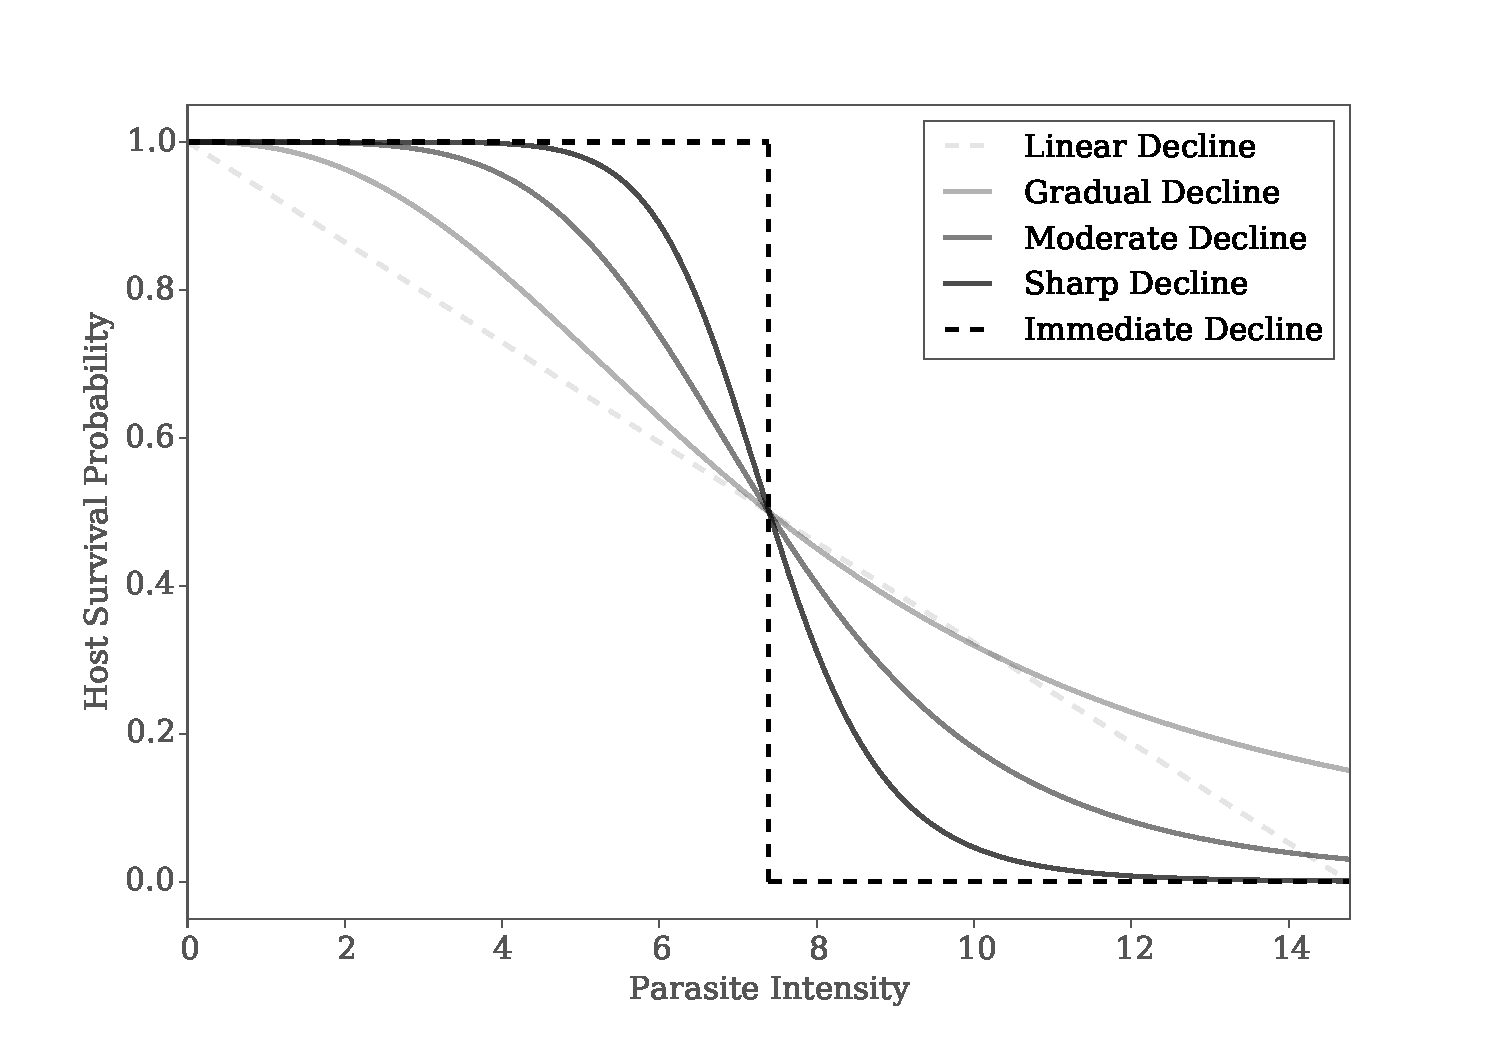
\includegraphics[width=\textwidth]{/Users/mqwilber/Repos/parasite_mortality/results/conceptual_fig.pdf}

    \caption{Five potential shapes for a host-survival functions. PIHM should be easier to detect for steeper host survival functions \citep{Lanciani1989}, but we may expect the bias in the parameter estimates to increase as it becomes increasingly difficult to distinguish between steep survival functions.}
    \label{fig:surv}
\end{figure}

\begin{figure}

    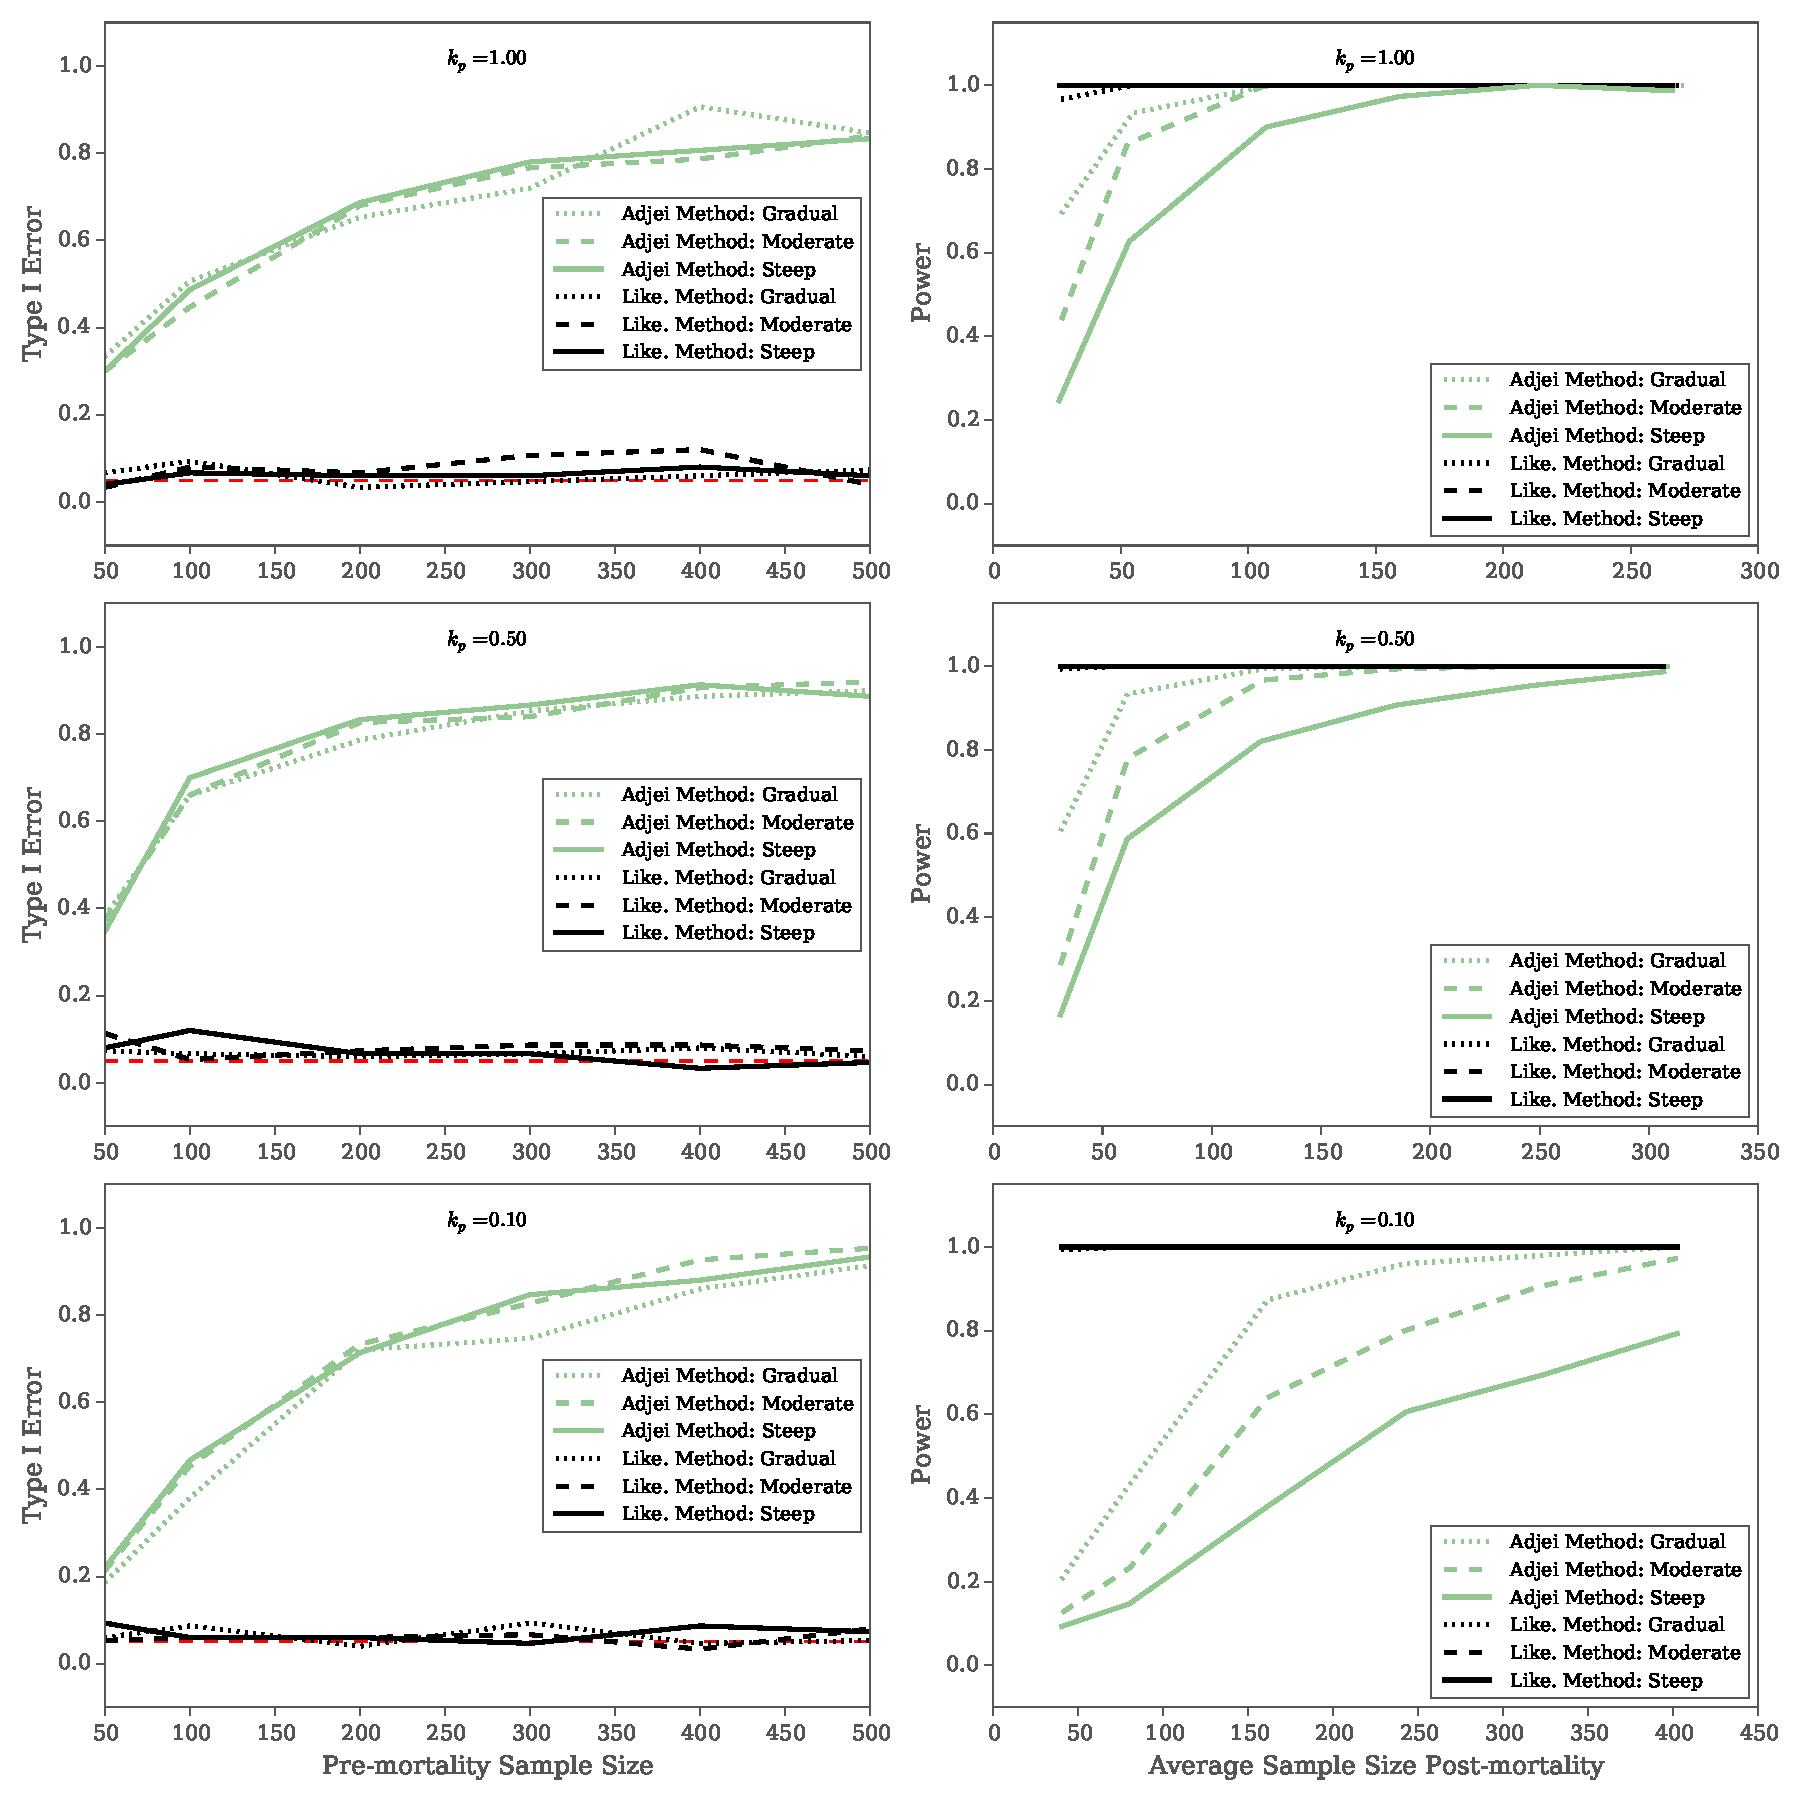
\includegraphics[width=\textwidth]{/Users/mqwilber/Repos/parasite_mortality/results/typeIpower_figure_for_mu10}

    \caption{The Type I error rate and the power of the Likelihood Method (solid line) and the Adjei Method (dashed lines) when $\mu_p = 10$ for various shapes of the host survival function and levels of aggregation $k_p$.  The first column gives the Type I error rate of each method for falsely detecting PIHM when none is present.  The red line gives the the pre-set Type I error rate of $\alpha = 0.05$.  The second column gives the power of a given method to detect PIHM when it is actually occurring. }
    \label{fig:typeI10}

\end{figure}


\begin{figure}

    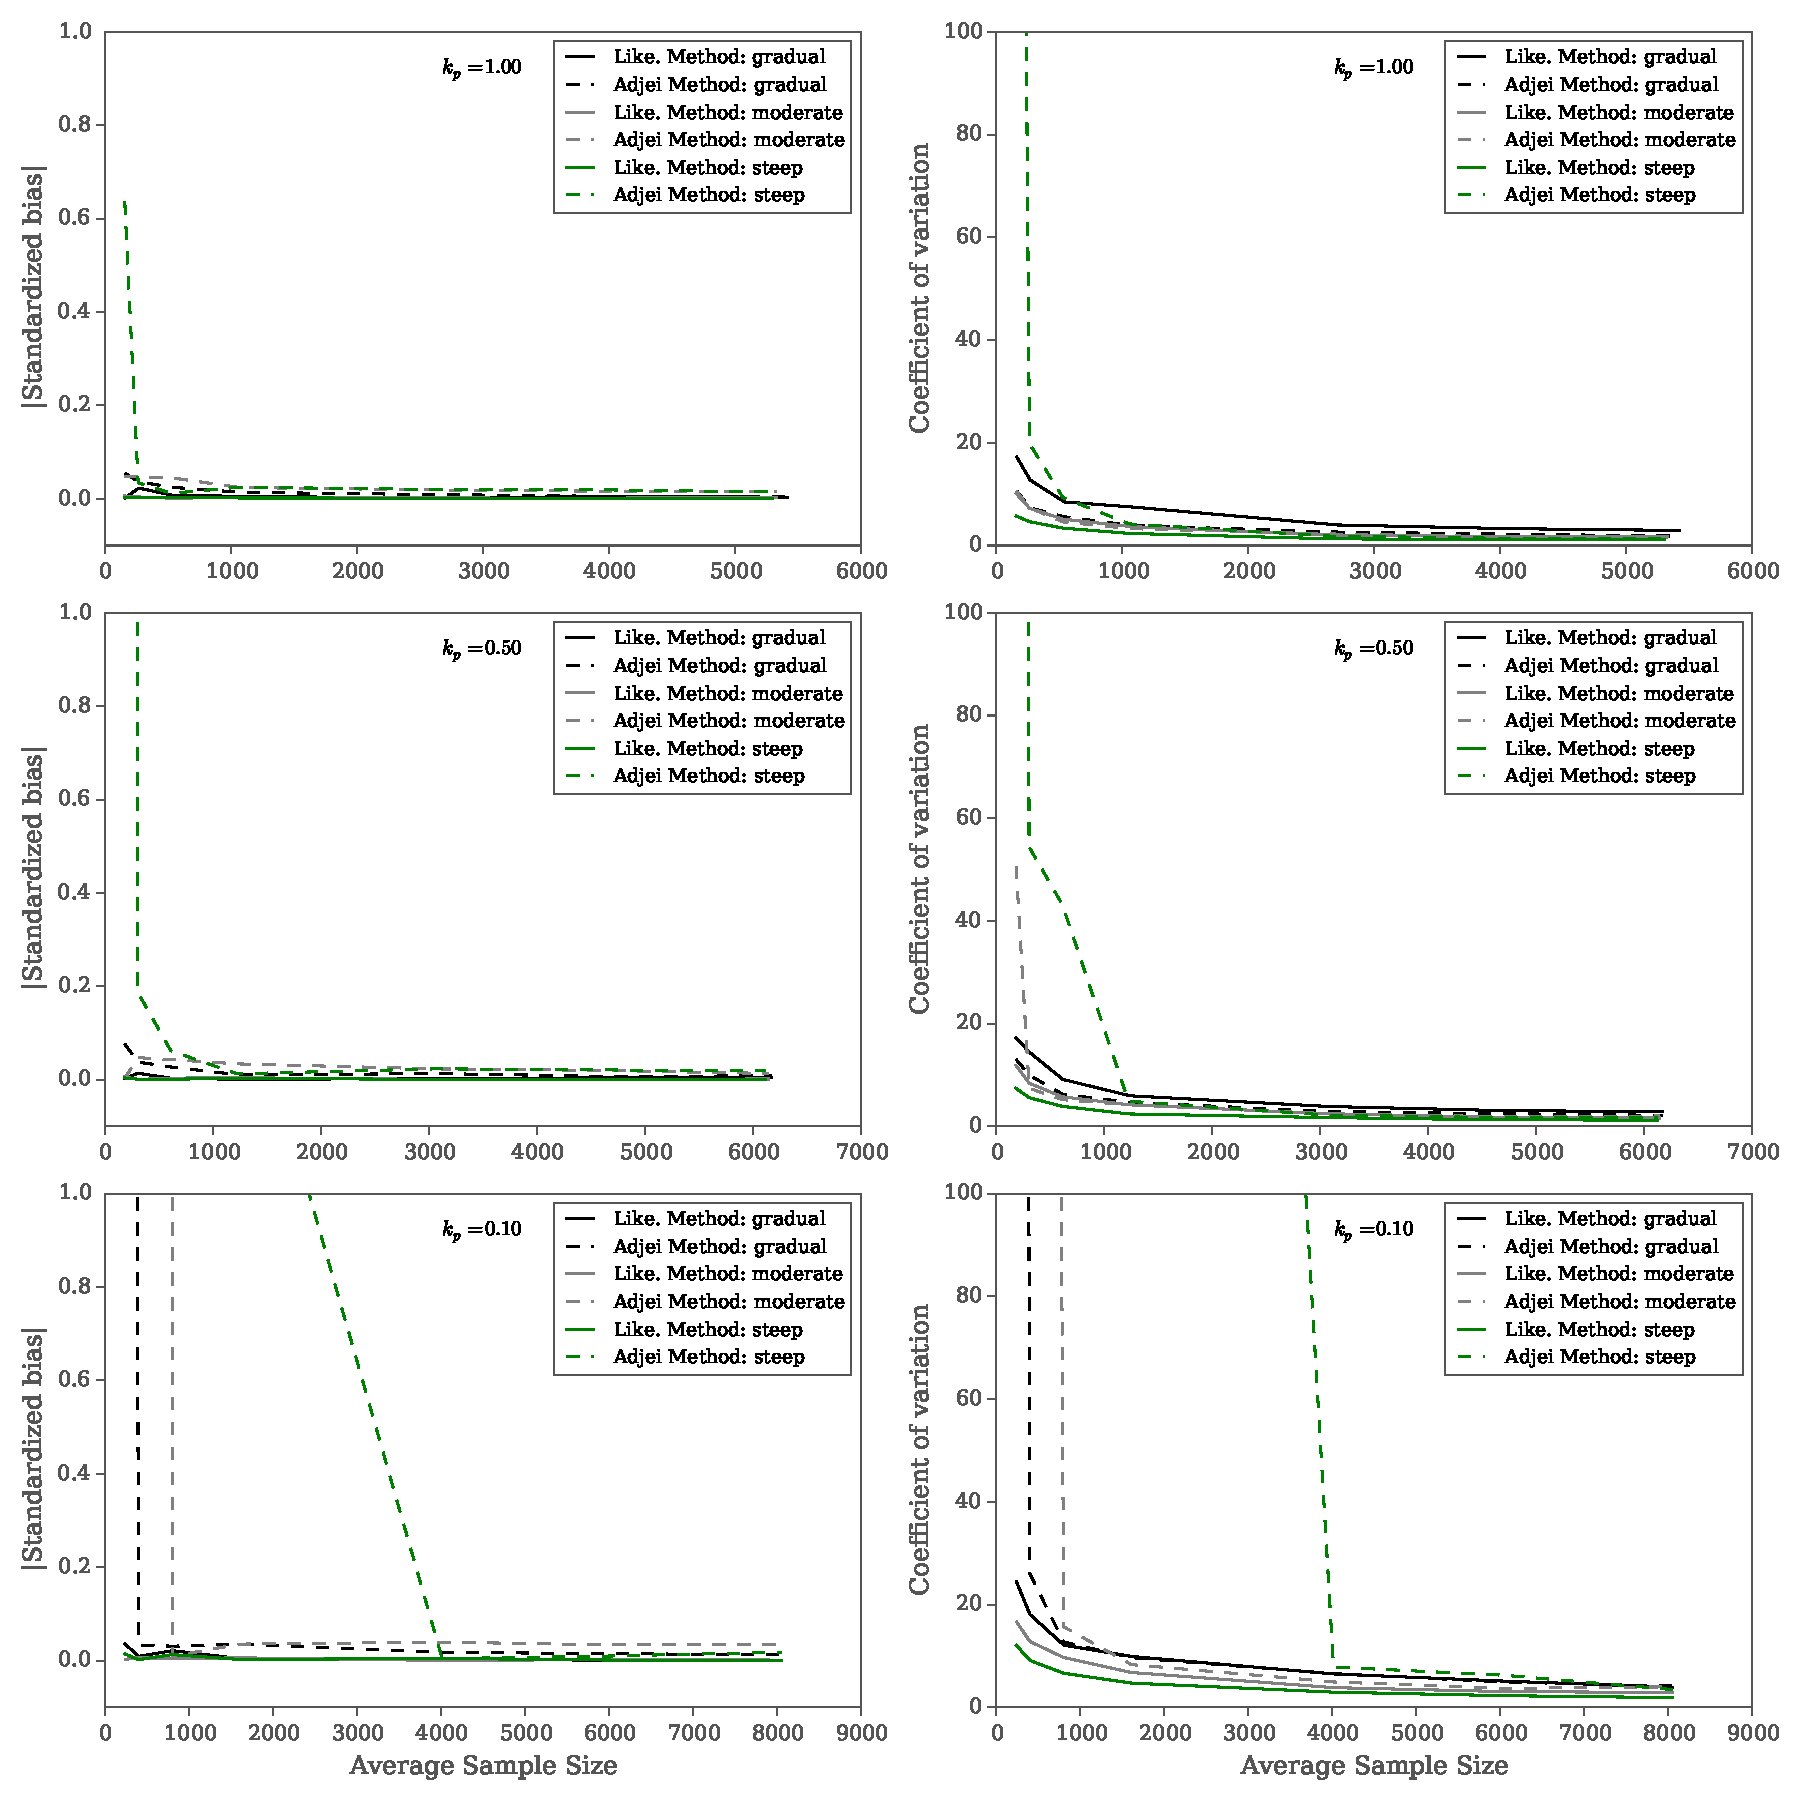
\includegraphics[width=\textwidth]{/Users/mqwilber/Repos/parasite_mortality/results/bais_prec_figure_for_ld50_mu10}

    \caption{The bias and the precision of the Likelihood Method (solid line) and the Adjei Method (dashed lines) when $\mu_p = 10$ for various shapes of the host survival function and levels of aggregation $k_p$ when estimating $LD_{50}$.  The first column gives the bias of each method's $LD_{50}$ estimate over 150 simulations. The second column gives the precision of each method's $LD_{50}$ estimate over 150 simulations.}

    \label{fig:biasld50}

\end{figure}

\begin{figure}

    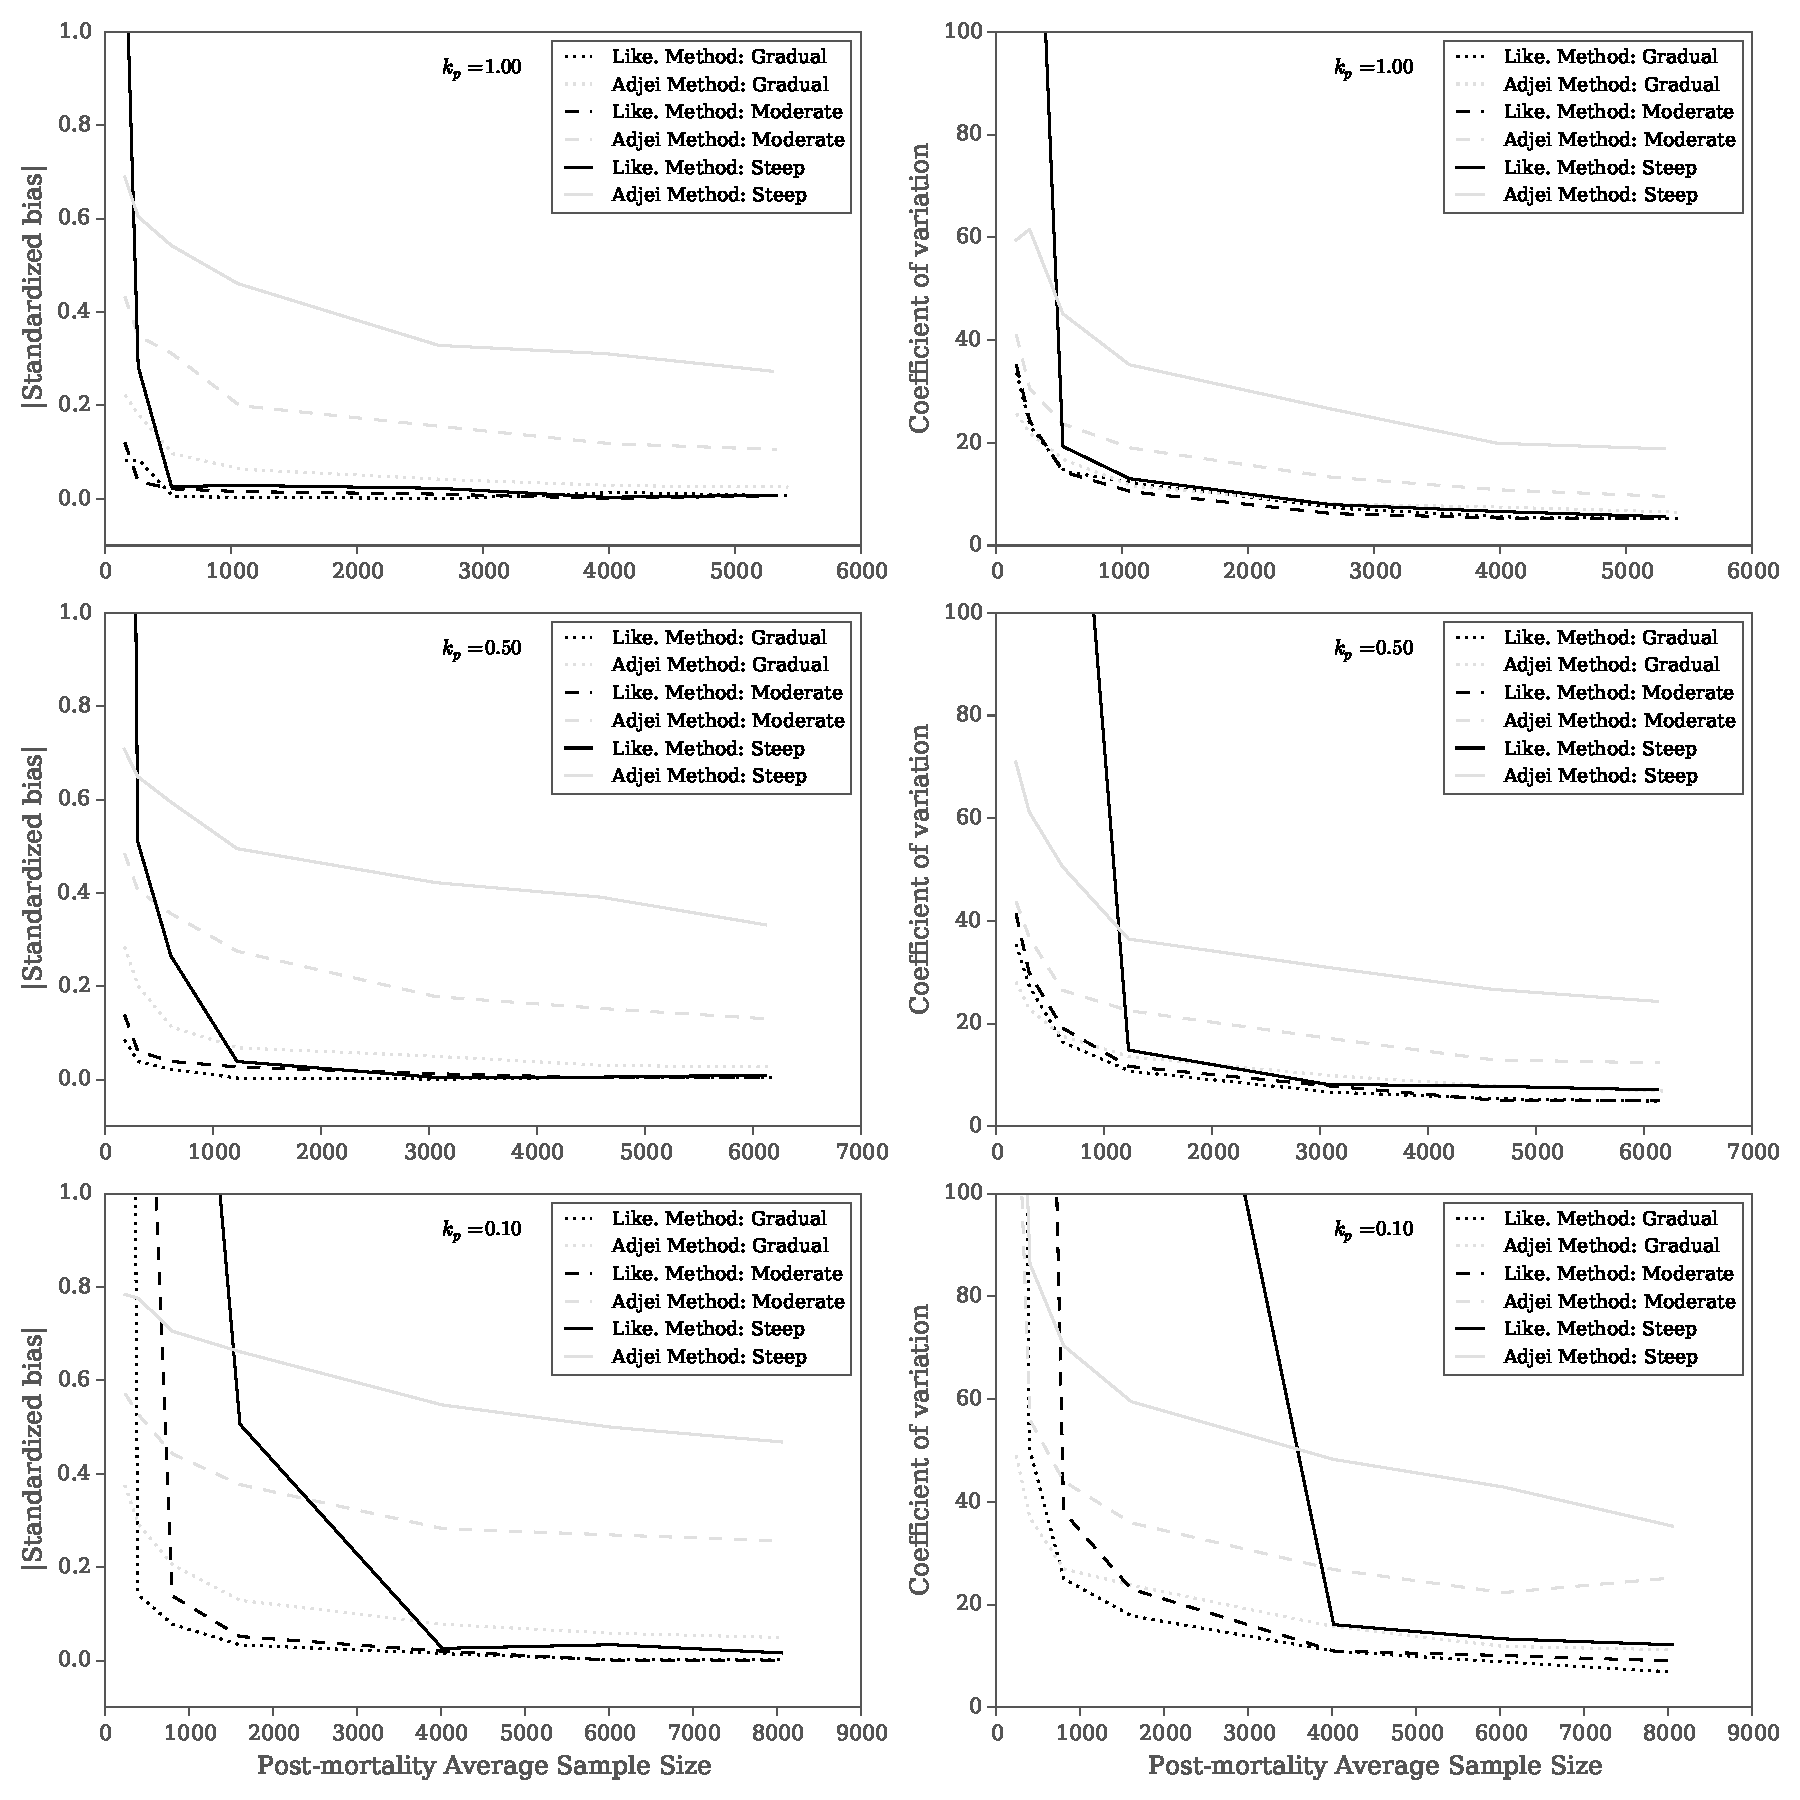
\includegraphics[width=\textwidth]{/Users/mqwilber/Repos/parasite_mortality/results/bais_prec_figure_for_a_mu10}

    \caption{The bias and the precision of the Likelihood Method (solid line) and the Adjei Method (dashed lines) when $\mu_p = 10$ for various shapes of the host survival function and levels of aggregation $k_p$ when estimating the $a$ parameter of the host survival function.  The first column gives the bias of each method's $a$ estimate over 150 simulations. The second column gives the precision of each method's $a$ estimate over 150 simulations.}

    \label{fig:biasa}

\end{figure}




\end{document}

